\section*{Task 1 : Writing Domain and Problem}
\thispagestyle{empty}

The aim of this fourth lab is to learn how to model a problem that can be
solved with automatic solvers called planners, using a formal language : PDDL.

Different domains alternatives are suggested. I have chosen to implement the AI
classic Shakey's World.

Shakey is a robot with two grippers that is moving in a set of rooms, connected
by doors. Each room contains a lightswitch which can be on or off but may also
contain big boxes or smaller objects.

The lab page defines the following constraints :
\begin{itemize}
  \item Shakey can carry small objects, but only two at a time because he has
  only two grippers.
  \item For Shakey to be able to find a small object in a room, the light must
  be on in that room.
  \item Shakey can not carry boxes, but can push them around. Boxes can only be
  pushed through wide doors, not narrow ones.
  \item To switch the light in a room on or off Shakey must climb onto a box
  that is positioned below the switch (otherwise he can not reach the switch).
  This may in turn require moving the box into position, possibly from another
  room.
\end{itemize}

\begin{center}
  \begin{verbatim}
  -------------------------------------------------------------------------
  |                       |                       |                       |
  |                       |                       |                       |
  |       light switch 1 -|- light switch2        |- light switch3        |
  |                       |                       |                       |
  |       ---             |                     door2                     |
  |       | |           door1      shakey         |                       |
  |       ---           (wide)                    |                       |
  |       box             |                       |                       |
  |                       |                     door3                     |
  |                       |                     (wide)                    |
  |        room1          |        room2          |         room3         |
  -------------------------------------------------------------------------
  \end{verbatim}
  SRI Shakey's World
\end{center}

The following actions have been implemented in the domain definition file :
move, push, climb, descend, turnon and pickup and drop.

A few assumptions have been made :
\begin{itemize}
  \item Doors are either opened wide or narrow, it is not possible to change the
opening.
  \item Shakey pushing a box from a room to another imply Shakey also being in
the destination room.
  \item When Shakey is on a box, he can only turn a light on, he has to reach
the ground before being able to move.
\end{itemize}

Please refer to the code and comments for more details regarding the
implementation.

\newpage
\thispagestyle{empty}
\subsection*{Testing the domain with a simple problem}

The example below is very simple problem just to test the domain.
Shakey is in room-1 and must bring the ball from room-1 to room-3 and then
go back to room-1. A climbable box is in room-1.

The goal is defined as follow :
\begin{verbatim}
(:goal (and(in ball room-3) (in shakey room-1 )))
\end{verbatim}

Using \textit{vhpop} planner on this simple problem we get the following
solution :

\begin{figure}[h]
    \centering
      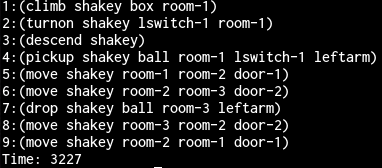
\includegraphics[width=0.50\linewidth]{./images/prob0_seq.png}
    \caption{Actions sequence using vhpop}
\end{figure}

\section*{Task 2 : Problems and performance comparison}
\thispagestyle{empty}
In this part we are going to test and compare the different planners on a range
of problems with increasing difficulty.

\begin{itemize}
  \item World dimensions : the default domain (see page 1) is composed of only
three rooms. If we add more rooms or change the disposition to a grid of (n,m) rooms, the complexity increases rapidly.
  \item The number of objects :
  \item The initial state :
\end{itemize}

\subsection*{Identifying parameters}
In order to create this range of problem, we first have to identify the
parameters that can be modified to scale up the difficulty.

\subsection*{Problems}



\subsection*{Results}

\textit{Test protocol : all tests have been done in the same conditions, on
the same computer.}

Now, let us consider the following test cases.
